% !TeX document-id = {412070ce-2b89-4575-900e-e9d3183d0ba4}
% !TeX TXS-program:bibliography = txs:///biber
\documentclass[unknownkeysallowed]{beamer}
\usetheme{UniKlu}
\usepackage[backend=biber,style=apa,sorting=nty, bibencoding=utf8]{biblatex}
\addbibresource{/home/donkarlo/Dropbox/projs/research/refs.bib}


\usepackage{xcolor}

\title{From Individual Perception to Collective Behavior in MAV. A self-aware approach}
\author{Mohammad Rahmani}
\institute{Pervasive Computing Group}

\begin{document}
	\begin{frame}
		\date{}
		\maketitle
		\textcolor{white}{\textbf{6 October 2020}}
	\end{frame}
	
	\begin{frame}{Intelligent Agents (IA), Sensors and Actuators}
		Each IA, either biological or artificial, incorporates:
		\begin{itemize}
			\item Sensors
				\begin{itemize}
					\item Proprioceptive (Cochlea, IMU)
					\item Exteroceptive (Eyes, Camera)
				\end{itemize}
			\item Actuators (Feet, Engine)
		\end{itemize}
	\end{frame}

	\begin{frame}{Self-awareness (SA)}
		SA is an approach in AI to enable IAs making a distinction between their \textbf{previous} experiences (The first one forms the initial knowledge) and new experiences observed by the sensors (\textbf{Abnormality detection}) \footnote{\fullcite{regazzoni-2020-multi-sensorial-generative-and-descriptive-self-awareness-models-for-autonomous-systems}} and
		\begin{itemize}
			\item build predictive generalized state models from these new experiences 
			\item store them and retrieve them to predict and plan future motions
			\item make appropriate decisions such as disturbance rejection or motion re-planning via actuators
		\end{itemize}
	\end{frame}

	\begin{frame}{Simple illustration of an SA drone}
		\begin{figure}
			\includegraphics[scale=0.06]{/home/donkarlo/Dropbox/projs/research/assets/sa-drone.png}
			\caption{SA, sensors and actuators}
		\end{figure}
	\end{frame}

	\begin{frame}{The ultimate goal of a self-aware IA}
		\begin{itemize}
			\item To maintain its homeostasis condition over the course of time by taking advantage of the modeled experiences to predict future states in order to plan and act accordingly to improve
			\begin{itemize}
				\item Resource management
				\item Security
				\item Safety
			\end{itemize}
		\end{itemize}
		\textbf{For this proposal embodies in \textbf{Collision avoidance}}
	\end{frame}

	\begin{frame}{Existing dynamic models on continuous generalized state space}
		\begin{itemize}
			\item DBN = A Markov chain that each of its state nodes is predicted by a bank of KFs 
		\end{itemize}
	\end{frame}

	\begin{frame}{Reference scenario in classical models}
		\begin{figure}
			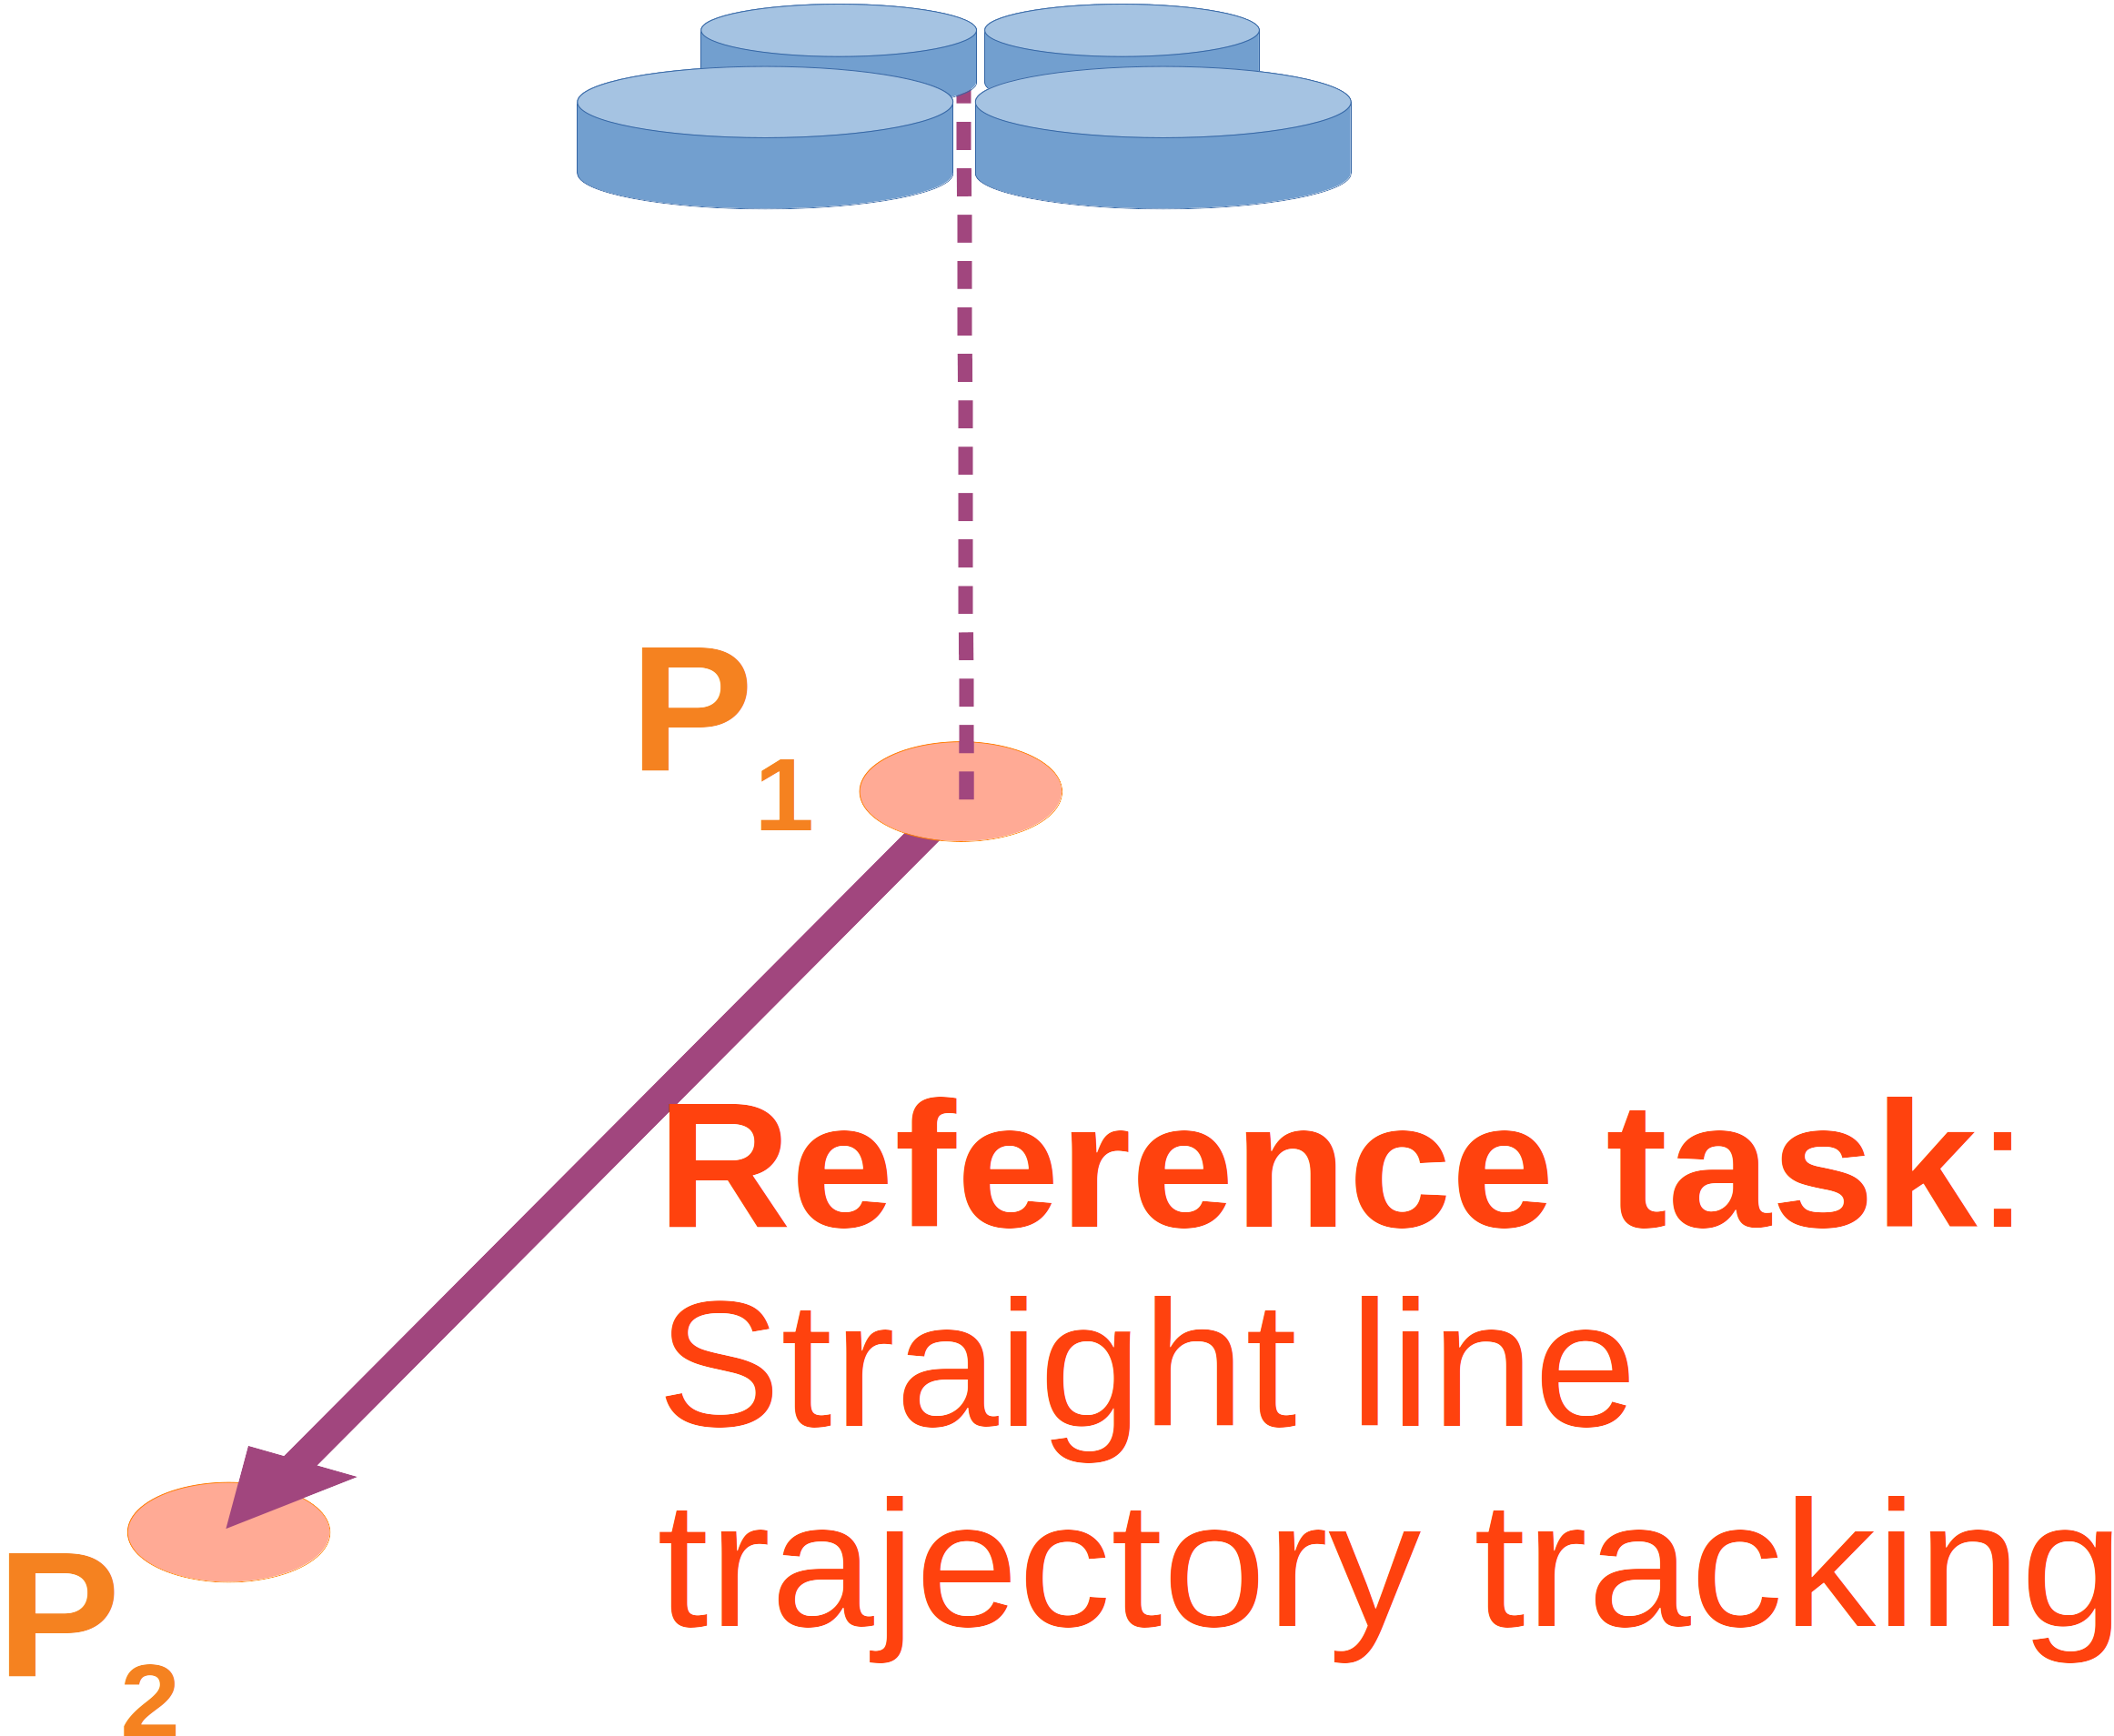
\includegraphics[scale=0.04]{/home/donkarlo/Dropbox/projs/research/assets/single-drone-reference-scenario.png}
		\end{figure}
	\end{frame}

	\begin{frame}{Force field theory and the obstacles to overcome in classical models}
		\begin{figure}
			\includegraphics[scale=0.04]{/home/donkarlo/Dropbox/projs/research/assets/single-drone-force-fields.scenarios.png}
		\end{figure}
	\end{frame}

	\begin{frame}{All experiences}
		\begin{figure}
			\includegraphics[scale=0.05]{/home/donkarlo/Dropbox/projs/research/assets/single-drone-all-scenarios.png}
		\end{figure}
	\end{frame}

	\begin{frame}{First language: Building a switching, predictive models for each individual agent}
		Discretized generalized state for different derivatives of time, forms the alphabet of words by which each individual agent can describe the experiences it is practicing to other agents \footnote{\fullcite{kanapram-2019-self-awareness-in-intelligent-vehicles-experience-based-abnormality-detection}}
		\begin{figure}
			\includegraphics[scale=0.4]{/home/donkarlo/Dropbox/projs/research/assets/trait-based-alphabets.jpg}
			\caption{}
		\end{figure}
		\begin{equation}
		w = \{\alpha^{(0)},...,\alpha^{(L)}\}
		\end{equation}
	\end{frame}

	\begin{frame}{First language: Discretization technique}
		Discretization
		\begin{itemize}
			\item GNG \footfullcite{fiser-2013-growing-neural-gas-efficiently}
			\begin{itemize}
				\item Online
			\end{itemize}
		\end{itemize}
	\end{frame}

	\begin{frame}{Reference and Vertical obstacle avoidance in the first language}
		\begin{figure}
			\includegraphics[scale=0.04]{/home/donkarlo/Dropbox/projs/research/assets/single-drone-reference-vertical-scenarios.png}
		\end{figure}
	\end{frame}

	\begin{frame}{A novel dynamic switching models, MJPF}
		\begin{itemize}
			\item MJPF (DBN = Level 1: Bank of KF - Level 2: Bank of PF in each Markov chain state)
		\end{itemize}
		\begin{figure}
			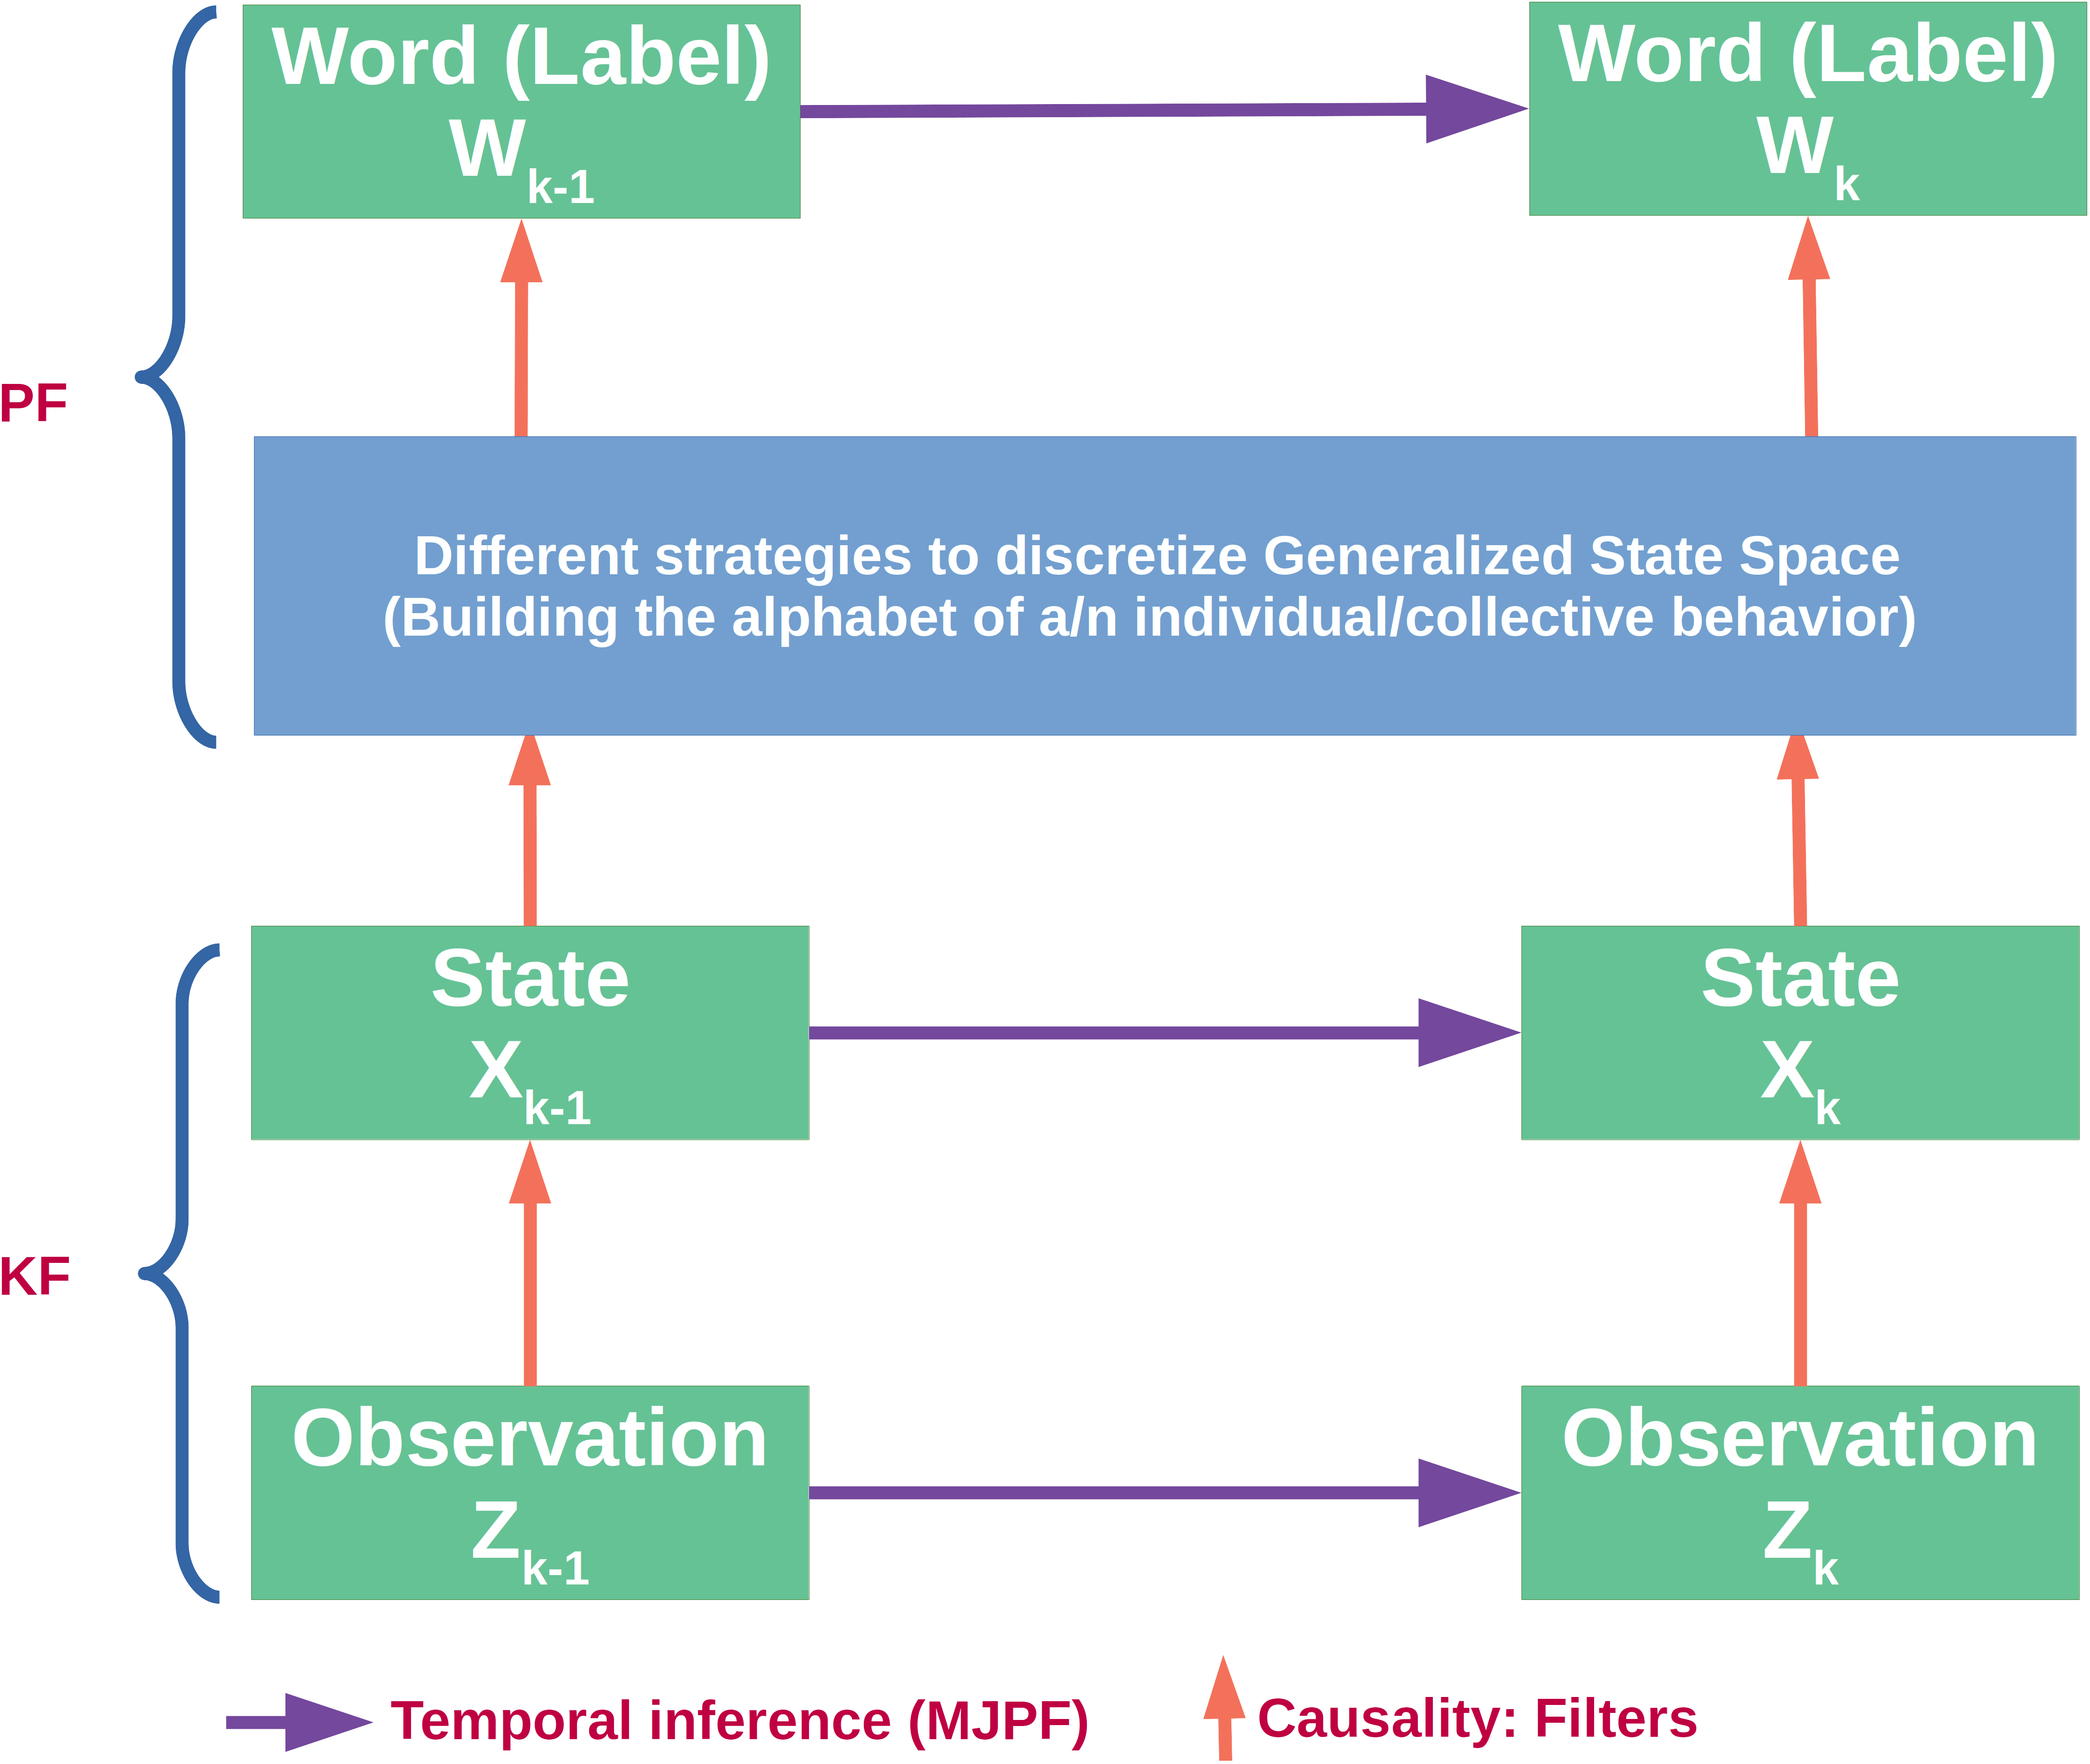
\includegraphics[scale=0.04]{/home/donkarlo/Dropbox/projs/research/assets/mjpf.png}
		\end{figure}
	\end{frame}

	\begin{frame}{Collective Self-awareness (CA)}
		\begin{itemize}
			\item The ability to detect abnormality in the course of relation that a collection of IAs were supposed to maintain to make appropriate decisions by the actuators to improve collective homeostasis conditions
			\begin{itemize}
				\item \textbf{Example}: Taking an appropriate \textbf{formation} when the collection faces a factor detrimental to its collective homeostasis condition
			\end{itemize}
		\end{itemize}
	\end{frame}

	\begin{frame}{CA in multi-MAV navigation for aerial manipulation}
		Not only each individual IA must be aware of new experiences observed from the environment, but also they must be able to detect anomaly in the motion of other agents in the collection.
	\end{frame}

	\begin{frame}{CA scenarios}
		CA formation models from which appropriate actions should be practiced
		\begin{figure}
			\includegraphics[scale=0.05]{/home/donkarlo/Dropbox/projs/research/assets/colletive-all-scenarios.png}
			\caption{}
		\end{figure}
	\end{frame}

	\begin{frame}{Second language: Describing the course of a collective behavior}
		Mutually activated discretized generalized state space form the collective language which can describe the expected behavior of a collection of agents are supposed to expose over a certain course of time \footnote{\fullcite{baydoun-2019-prediction-of-multi-target-dynamics-using-discrete-descriptors-an-interactive-approach}}
		\begin{figure}
			\includegraphics[scale=0.7]{/home/donkarlo/Dropbox/projs/research/assets/mutial-experienced-semantics.jpg}
			\caption{}
		\end{figure}
	\end{frame}

	\begin{frame}{Second language: Discretization technique}
		Discretization
		\begin{itemize}
			\item SOM \footfullcite{kohonen-2001-self-organizing-maps} or even a simple K-means
			\begin{itemize}
				\item Offline
			\end{itemize}
		\end{itemize}
	\end{frame}
	
	\begin{frame}{Continual/life long learning for both SA and CA}
		\begin{itemize}
			\item Variational Auto Encoders/Decoders (To generate different versions of the same experience)
			\item Continual/Lifelong learning (To include all experiences in one model)
			\item Define an abnormality tolerance level which adopts to newly added models
		\end{itemize}
	\end{frame}

	\begin{frame}{The main challenge}
		If each agent describes the following changes to it's neighboring agents
		\begin{itemize}
			\item  Generalized state described by the first language
			\item  Practicing predictive model trained by the first language
		\end{itemize}
		, then the main challenge is to train a model to
		\begin{itemize}
			\item map samples of the aforementioned populations to a sentence of the  second language 
		\end{itemize}
		\textbf{to find out how efficient such model can improve homeostasis level of individual agents and the whole system.}
	\end{frame}

	\begin{frame}{Simulation environment}
		\begin{itemize}
			\item ROS as robot simulation tool
			\item GAZEBO as simulation tool
			\item MAVLINK as communication standard
				\begin{itemize}
					\item MAVSDK ... Python implementation
				\end{itemize}
		\end{itemize}
	\end{frame}
\end{document}
